%		** MECCANISMO D'ASTA **

Le aste rappresentano l'elemento fondamentale dell'interazione fra gli agenti. Tramite le aste, gli agenti possono cedere e acquisire nuovi target da tracciare. Ci sono due momenti in cui un agente pu� bandire un'asta:
\begin{itemize}
	\item quando un target attualmente tracciato � in procinto di abbandonare la sua area di visione; in tal caso diremo che lo sta perdendo
	\item quando, dopo aver ricevuto notifica sulla vincita di un'asta precedente, cerca di cedere il target che gi� sta tracciando.
\end{itemize}
Il protocollo d'asta implementato prevede l'utilizzo di aste \textit{First-Price Sealed-Bid}: un tipo d'asta \textit{one-shot} a busta chiusa. 

Il valore della puntata di un'asta viene specificato attraverso la seguente funzione, la quale � implementata attraverso l'azione interna \textit{calculateBid}.

Siano $A$ l'agente che deve effettuare la puntata per il nuovo target $t_n$, $t$ l'eventuale target che $A$ sta gi� tracciando, $N_A$ il numero di vicini di $A$, $dist$ una funzione distanza (ad es. distanza Euclidea) fra un agente ed un target e $k \in \mathbb{N}$ tale che $k \gg \max dist(A, t)$, allora:
\begin{center}
	$$
	b(A) =
	\begin{cases} 	
	\frac{(2 dist(A,t) - dist(A, t_n))}{N_A} - k & \mbox{se }A \mbox{ sta tracciando }t \\ \\
	\frac{dist(A,t_n)^{-1}}{N_A} + k & \mbox{ altrimenti.}
	\end{cases} 
	$$
\end{center}
La funzione cos� definita soddisfa i seguenti vincoli:
\begin{itemize}
	\item gli agenti "liberi" vincono sempre sugli agenti "occupati"
	\item fra agenti "liberi" vince sempre il pi� vicino al target
	\item fra agenti "occupati" vince sempre l'agente che ha pi� vicino il target e contemporaneamente ha il target attualmente tracciato pi� lontano
	\item a parit� di tutto, vince chi ha meno vicini.
\end{itemize}

Una tipica interazione fra agenti in un contesto d'asta � rappresentata dal seguente \textit{sequence diagram}.

% Figura sequence diagram
\begin{figure}[htp]
	\centering
	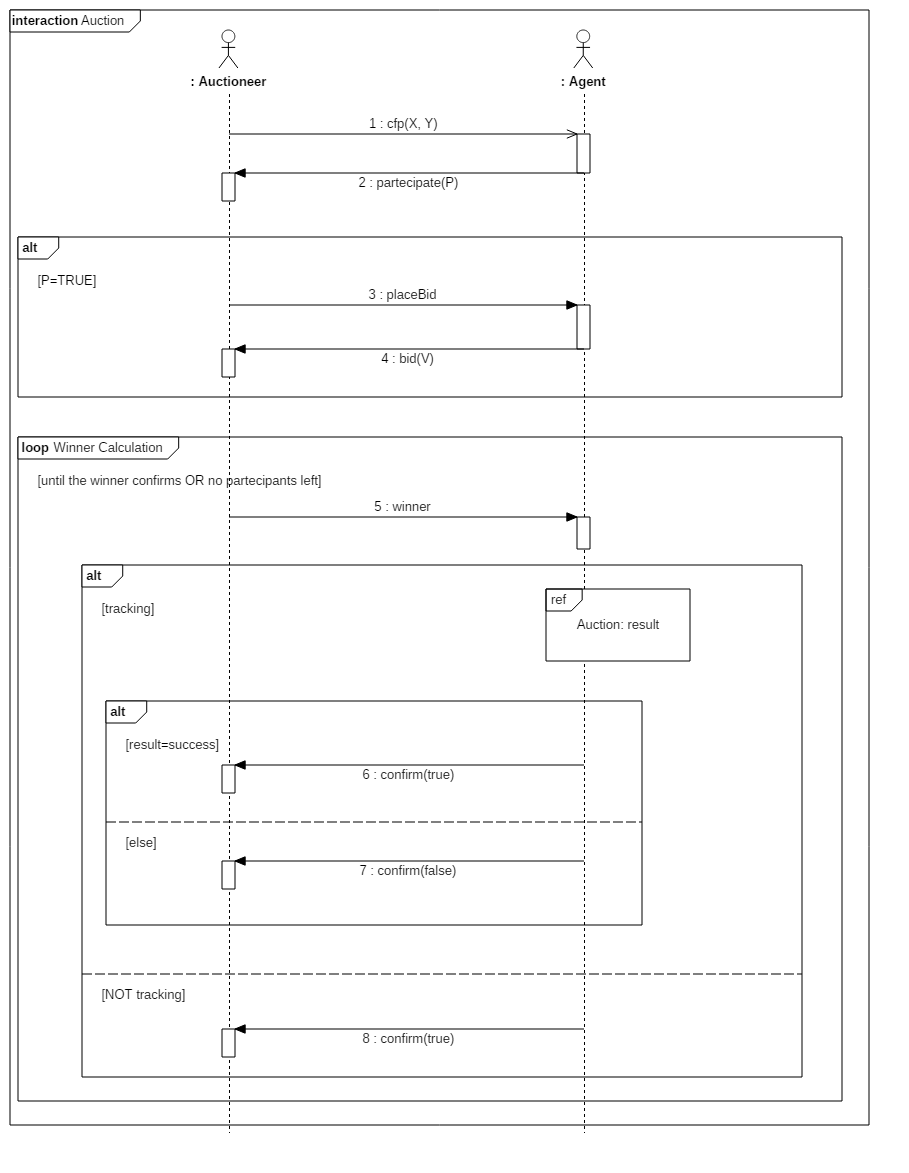
\includegraphics[width=\linewidth]{Auction}
	\caption{Protocollo d'asta.}
	\label{fig:auction}
\end{figure}

\newpage

Il protocollo prevede i seguenti passi.
\begin{itemize}
	\item Un agente che vuole cedere il suo target ricopre il ruolo di banditore e invia a tutti gli agenti una \textit{call-for-proposal} per informarli dell'asta.
	\item Gli agenti che hanno ricevuto la call-for-proposal rispondono al banditore se sono interessati all'asta oppure no.
	\item Il banditore chiede, solo agli agenti interessati, di fare un offerta.
	\item Gli agenti interessati calcolano l'offerta e la inviano al banditore.
	\item Il banditore, dopo aver ricevuto un'offerta da tutti gli agenti interessati, sceglie il vincitore (l'agente che ha fatto l'offerta dal valore pi� alto) e gli notifica la vincita.
	\item L'agente vincitore pu� trovarsi in due stati.
	\begin{itemize}
		\item Se � occupato a tracciare un altro target, bandisce un'asta per quest'ultimo e aspetta che questa si concluda; se la sua asta termina con successo, conferma la sua vincita al banditore, altrimenti rigetta la vincita.
		\item Se � libero, conferma semplicemente la vincita al banditore.
	\end{itemize}
	\item Il banditore, se ha avuto una conferma dal vincitore, gli affida il target; altrimenti, ricalcola il vincitore fra gli altri candidati; se non esistono altri agenti di questo tipo, allora l'asta fallisce ed il banditore non pu� affidare a nessuno il suo target.
\end{itemize}
